\subsection{Class Diagram}

\begin{figure}[!ht]
\centering
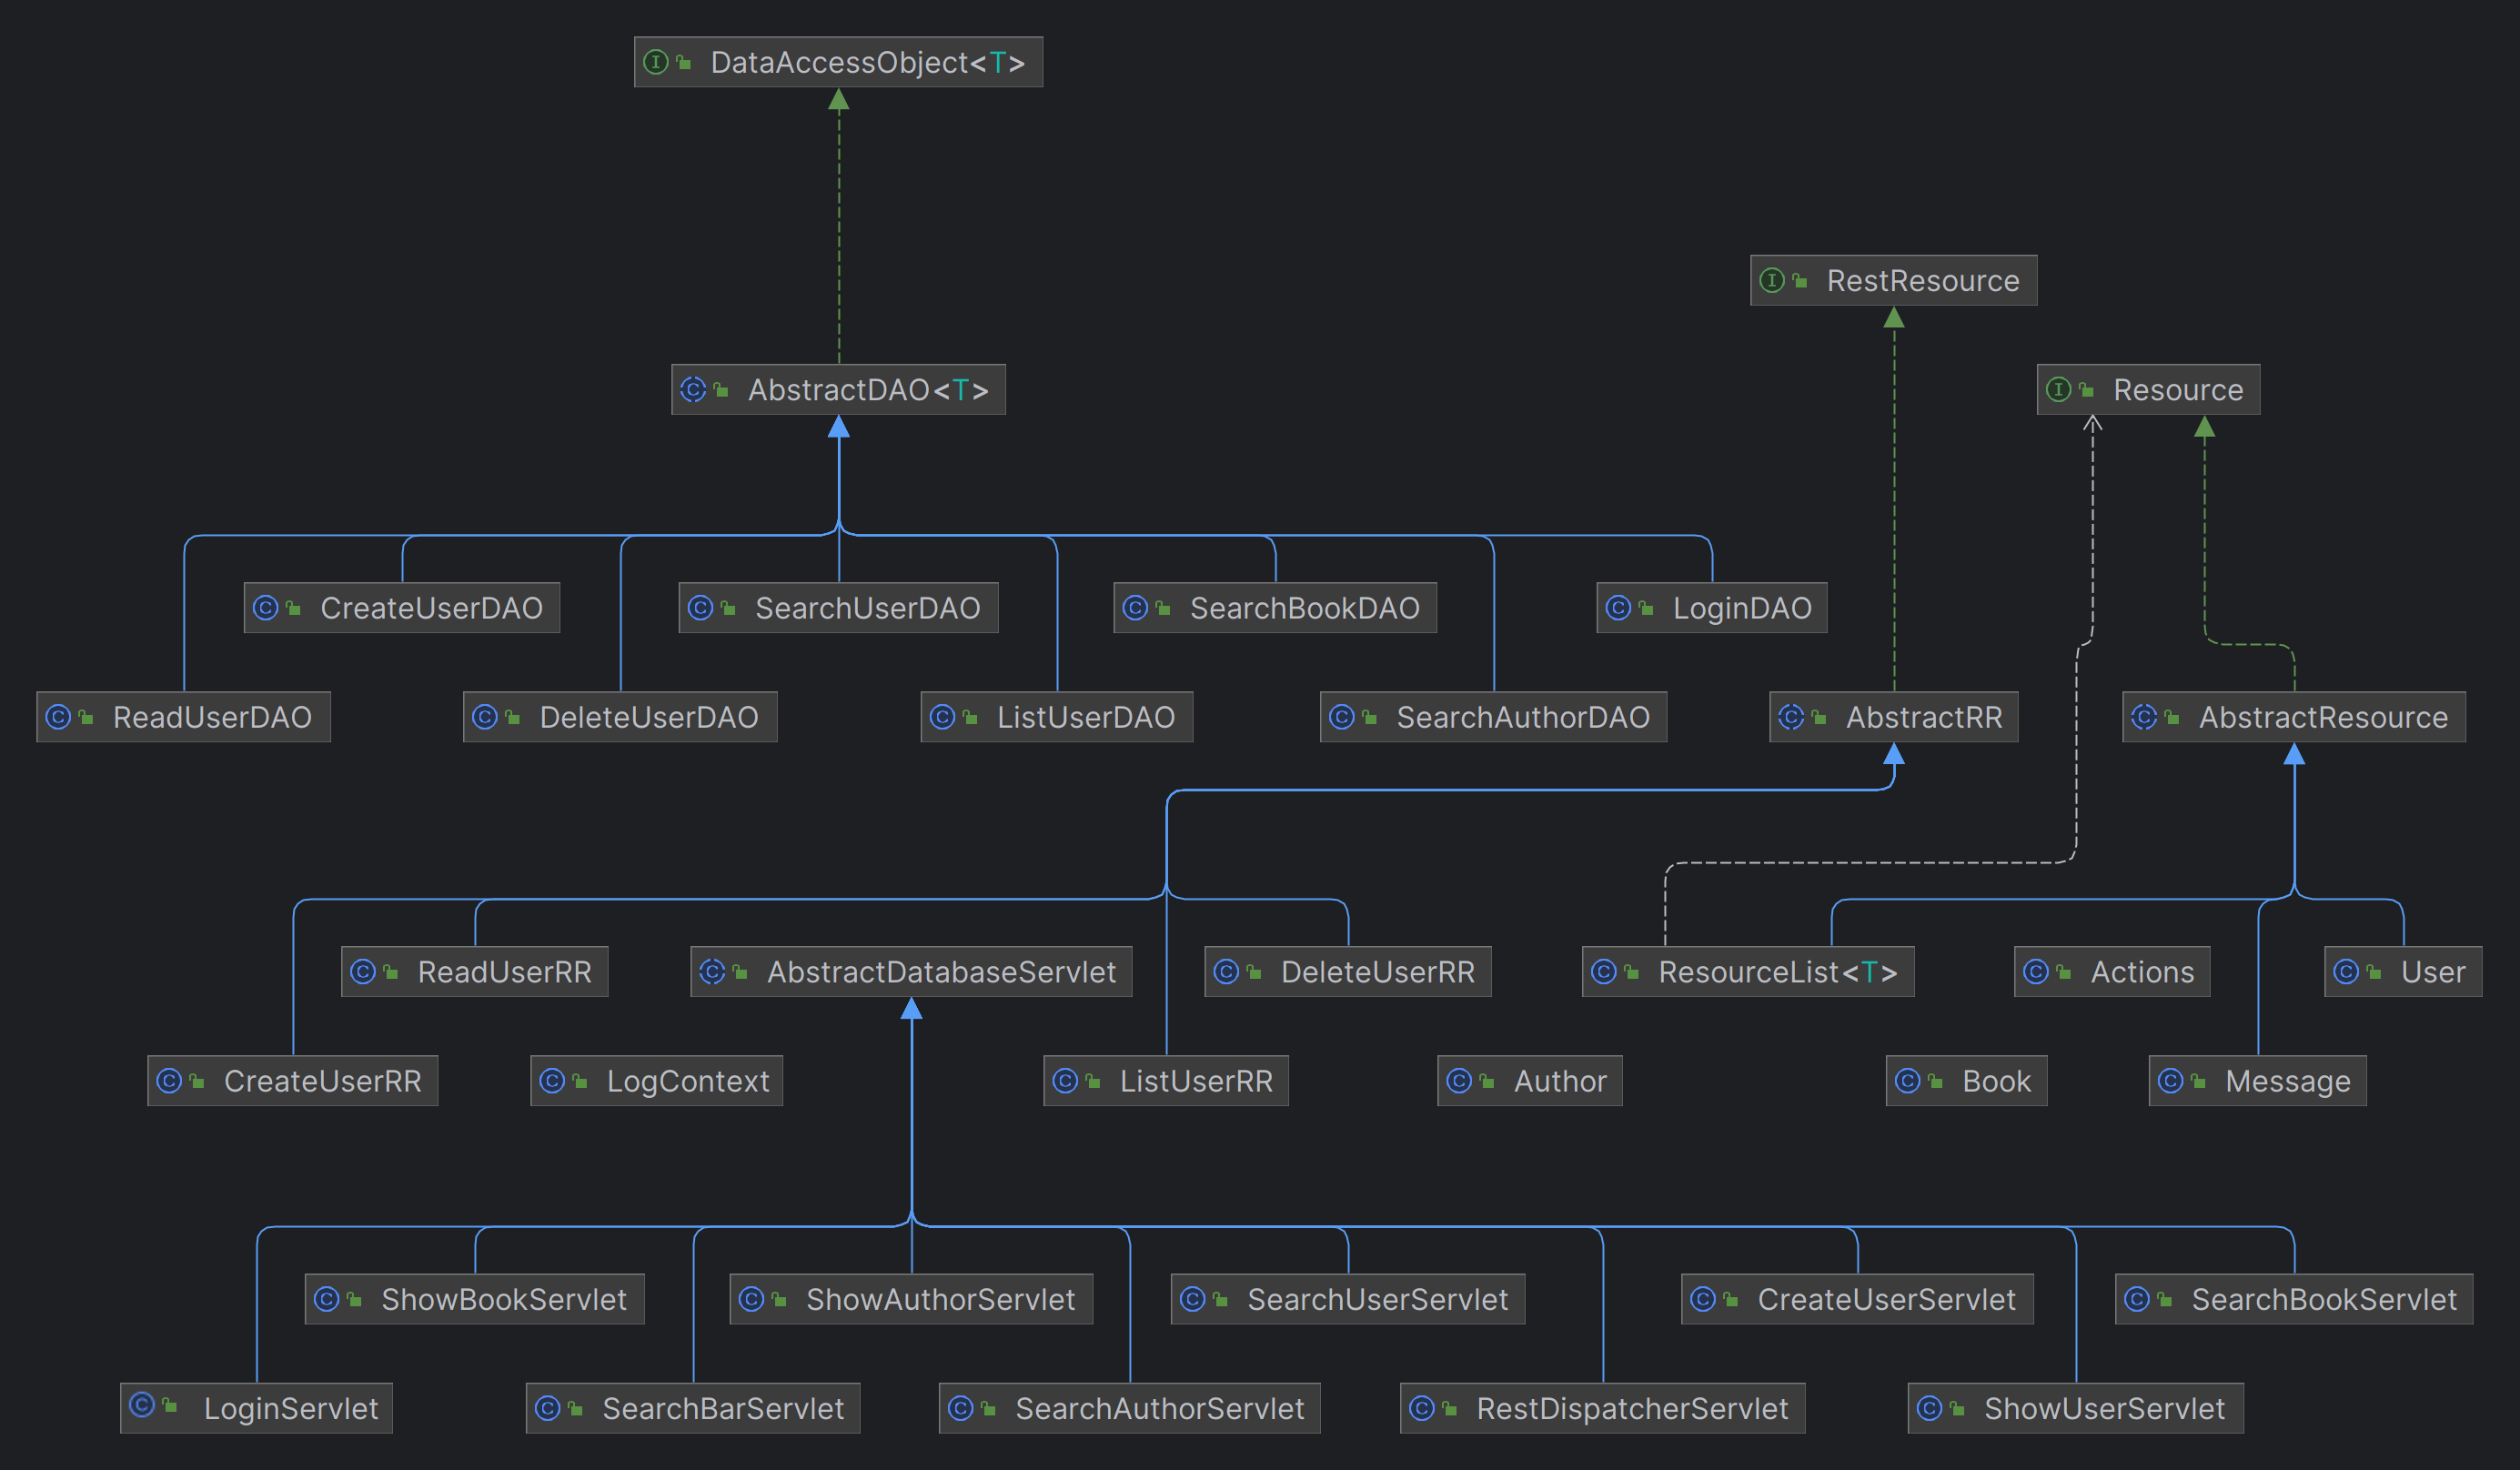
\includegraphics[width=0.85\textwidth]{sections/Class_diagram.png}
\caption{Class diagram of the book recommendation system}
\end{figure}

%Describe here the class diagram of your project
The class diagram represents the structure of a web-based application for managing users, books, and authors in a book recommendation system. The classes can be divided into the following categories:
\begin{itemize}
\item \textbf{Data Access Objects (DAO)}: This category includes abstract classes like AbstractDAO and concrete classes like CreateUserDAO, SearchUserDAO, SearchBookDAO, LoginDAO, ReadUserDAO, DeleteUserDAO, ListUserDAO, and SearchAuthorDAO. These classes handle data access operations related to users, books, and authors, such as creating, reading, updating, and deleting data.
\item \textbf{Resource Classes}: The `Resource` class and its subclasses `RestResource`, `AbstractRR`, and `AbstractResource` represent resources in the application, which could be related to users, books, authors, or other entities.

\item \textbf{Entity Classes}: Classes like `User`, `Book`, `Author`, `Actions`, `Message`, and `ResourceList` represent the entities or data models in the application.

\item \textbf{Servlet Classes}: Classes like `ShowBookServlet`, `ShowAuthorServlet`, `SearchUserServlet`, `CreateUserServlet`, `SearchBookServlet`, `LoginServlet`, `SearchBarServlet`, `SearchAuthorServlet`, `RestDispatcherServlet`, and `ShowUserServlet` are servlets that handle HTTP requests and responses, and interact with the DAO and resource classes to perform the required operations.

\item \textbf{Utility Classes}: Classes like `DataAccessObject`, `AbstractDatabaseServlet`, and `LogContext` provide utility functions or shared functionality across the application.
\end{itemize}

